\chapter{Introduction}\label{chapter:intro}
The way of transportation is in a transformation phase and autonomous driving technology is expected to have a big impact. Over one million people are killed in traffic-related accidents each year, where the vast majority of the accidents are caused by human mistakes~\cite{WHO2018, NHTSA2018}. 

Autonomous driving technology is expected to have a massive effect on the current transportation system and benefit society in many ways. For example, over one million people are killed in traffic-related accidents each year, where the vast majority of the accidents are caused by human mistakes~\cite{WHO2018, NHTSA2018}. By removing humans from the control of the vehicles, autonomous driving could significantly improve the traffic safety. Furthermore, the productivity of commercial heavy vehicles is increased when fewer human drivers are required, and the road infrastructure could be utilized more efficiently by scheduling transports outside of rush hours, for example during nights~\cite{FAGNANT2015167}.

Major progress towards deploying autonomous vehicles has been made during the last decade. The perception systems have been remarkably improved, largely due to the success of deep learning techniques~\cite{Janai2020}. The low-level control of the vehicle is a mature research area and can be solved with classical control theory methods~\cite{Paden2016}. However, how to approach the high-level decision-making in complex traffic situations is less explored and forms the main topic of this thesis.

\section{Problem Formulation}
The work presented in this thesis has in particular focused on the following research questions:
\begin{enumerate}
	\item[\textbf{Q1.}] How can RL be used to create a decision-making agent for autonomous driving, that can handle different intersection and roundabouts (complex urban scenarios)? Learn a scalable policy that is able to handle different scenarios. relative coordinate system. Action space. 
	(specificera for att komma undan varfor har du inte kollat pa andra metoder. How can we use RL for AD )
	\item[\textbf{Q2.}] How can AD domain knowlage (and models) be used to improve the action and state space for a RL agent? MPC for actions, Particle filter for intention distrubution. How can AD domain knowlage be used to create a state and action space that improves the RL agent?
	\item[\textbf{Q3.}] How can the quality of a RL agent be imporved by accounting for uncertainty?
	(How can the uncertainty of the RL agent be utilized?) (RPF-in the output and PF-in the input space)
\end{enumerate}



\begin{enumerate}
	\item We want to drive through intersections. 
	\item The intersection can be of different shapes. We assume we have a map of the intersection. 
	\item There will be other cars crossing the same intersection. 
	\item We have access to sensors on-board the ego vehicle. 
	\item We dont assume any knowlage of traffic signs or traffic lights. 
	\item We dont have v2v, or v2x communication. 
	
	To compensate for not having v2v or v2x communitaion, we have to predict what other driver will do. 
	
\end{enumerate}



\subsection{Scope / Limitations}
FILL

\subsection{System Architecture}
outline system architecture and limit this papre to comfortable decisions 

\begin{figure}[t]
	\centering
	\mbox{\parbox{\textwidth}{
			\centering
			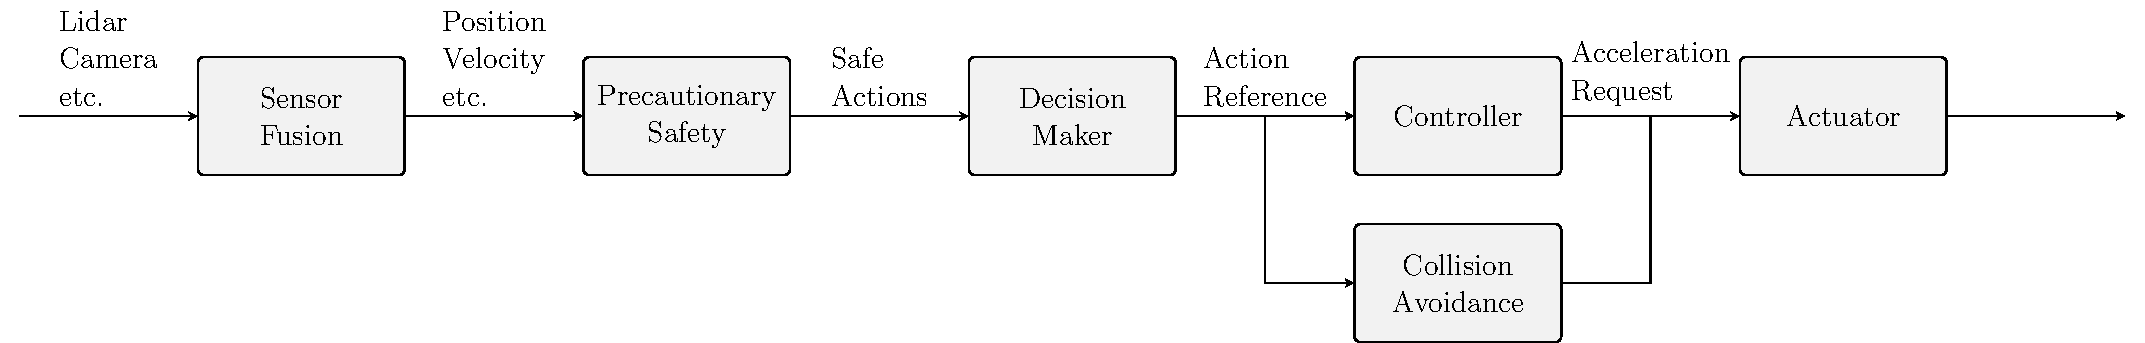
\includegraphics[width=\linewidth]{YourThesis/chapters/figures/pomdp/figures-system_architecture.pdf}%We suggest that you use a text box to insert a graphic (which is ideally a 300 dpi TIFF or EPS file, with all fonts embedded) because, in an document, this method is somewhat more stable than directly inserting a picture.   
	}}
	\caption{Representation of the system architecture.
	}
	\label{fig:systemArchitecture}
\end{figure}

\subsection{Contributions}

The main contributions of this thesis are:
\begin{enumerate}
	\item FILL

\end{enumerate}


\section{Thesis Outline}
FILL


